\documentclass[onecolumn, draftclsnofoot,10pt, compsoc]{IEEEtran}
\usepackage{graphicx}
\usepackage{url}
\usepackage{setspace}
\usepackage{caption}

\graphicspath{ {images/} }

\usepackage{geometry}
\geometry{textheight=9.5in, textwidth=7in}

\def \CapstoneTeamName{		Look Boss, No Hands}
\def \CapstoneTeamNumber{		9}
\def \GroupMemberOne{			Brandon Dring}
\def \GroupMemberTwo{			Nipun Bathini}
\def \GroupMemberThree{			Carl Benson}
\def \CapstoneProjectName{		CDK Global: No more touch. No more Keyboard. Bring it All Together. Using Technology to Teach Humans.}
\def \CapstoneSponsorCompany{	CDK Global}
\def \CapstoneSponsorPerson{		Trevor moore}


\def \DocType{Design Document}

\newcommand{\NameSigPair}[1]{\par
\makebox[2.75in][r]{#1} \hfil 	\makebox[3.25in]{\makebox[2.25in]{\hrulefill} \hfill		\makebox[.75in]{\hrulefill}}
\par\vspace{-12pt} \textit{\tiny\noindent
\makebox[2.75in]{} \hfil		\makebox[3.25in]{\makebox[2.25in][r]{Signature} \hfill	\makebox[.75in][r]{Date}}}}


%%%%%%%%%%%%%%%%%%%%%%%%%%%%%%%%%%%%%%%
\begin{document}
\begin{titlepage}
    \pagenumbering{gobble}
    \begin{singlespace}
        \hfill
        \par\vspace{.2in}
        \centering
        \scshape{
            \huge CS Senior Capstone \DocType \par
            {\large December 1st, 2017}\par
            \vspace{.5in}
            \textbf{\Huge\CapstoneProjectName}\par
            \vspace{.5in}
              
            \vfill
            {\large Prepared for}\par
            \Huge \CapstoneSponsorCompany\par
            \vspace{5pt}
            {\Large\NameSigPair{\CapstoneSponsorPerson}\par}
            {\large Prepared by }\par
            Group\CapstoneTeamNumber\par
            % 5. comment out the line below this one if you do not wish to name your team
            \vspace{0.2cm}
            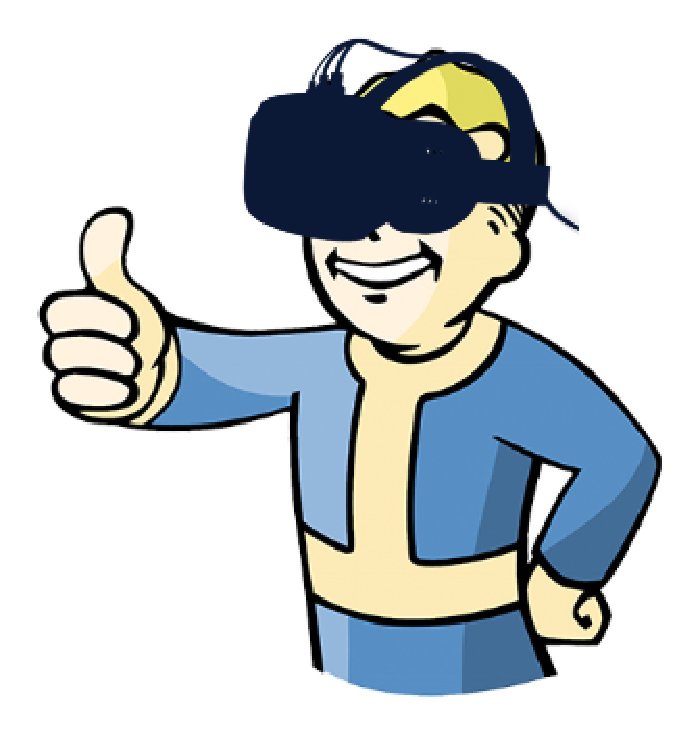
\includegraphics[height=4cm]{Team_logo}\\
            \vspace{0.2cm}
            \CapstoneTeamName\par
            \vspace{5pt}
            {\Large
                \NameSigPair{\GroupMemberOne}\par
                \NameSigPair{\GroupMemberTwo}\par
                \NameSigPair{\GroupMemberThree}\par
            }
            \vspace{20pt}
        }
        \begin{abstract}
        % 6. Fill in your abstract
       The purpose of this document is to go over in-depth architecture and design decisions for our project Look Boss, No Hands. Throughout, we will go over whom this project is meant for, the general components and their structure, along with the functional role each piece of technology and hardware plays in the project, and the rationale as to why they were designed in such a way. 


        \end{abstract}
    \end{singlespace}
\end{titlepage}
\newpage
\pagenumbering{arabic}
\tableofcontents
\clearpage

\section{Distribution of Work}
All group members contributed to each section rather than individually producing specific portions.

Brandon Dring:
\begin{itemize}
    \item \LaTeX \hspace{2pt}formatting %FANCY!
    \item Introduction
    \item System Overview
    \item System Architecture
    \item VR User Interface
    \item Build Stages
\end{itemize}
Carl Benson
\begin{itemize}
    \item Introduction
    \item System Overview
    \item Components
\end{itemize} 
Nipun Bathini
\begin{itemize}
    \item Define Alexa and AWS
    \item Alexa Components 
    \item AWS components 
\end{itemize}

\section{Introduction}
    \subsection{Scope}
        We will discuss the development of the core design elements of Look Boss, No Hands. It will include the relationship between components, specific technologies, and design viewpoints for each.
        
    \subsection{Purpose}
        To specify the content and organization of the core design elements of this project. It will include descriptions, implementation methods, and multiple viewpoints for each of these design elements.
        
    \subsection{Intended Audience}
        Intended for developers, clients, and managers of the Look Boss, No Hands project. It guides the designers in the selection, organization, and implementation of the design information. For the clients and managers of the project it will provide a guide for future development in the upcoming months.
        
    \subsection{Definitions}
        \begin{itemize}
            \item Alexa: Voice assistant from Amazon that interprets natural language commands and sends them to Lambda for processing. 
            \item Amazon Web Services (AWS): Cloud based computing platform that offers server hosting with an efficient, secure, reliable, and economical focus. 
            \item Lambda: Anonymous server functionality that processes commands and actions requested by Alexa with AWS. 
            \item VR: Virtual reality environment one can slip into by putting on a headset. 
            \item GameObject: An attribute that you can put on an object in VR to give it certain characteristics like textures, colors, interaction methods, etc. 
            \item Intent: Custom commands that are mapped to a specific query by the Alexa from the users voice.
            \item Abstraction: Creating a layer around an object to hide the low level details and complexity thus, allowing for easier, and higher level use. 
            \item JSON: Javascript Object Notation, a data format contained within a single object accessed via the {'}.{'} operator. Possible formats include other objects, arrays, strings, and numbers. 
            \item MongoDB: A noSQL type of database, in which the entire file is stored as a giant JSON object. 
        \end{itemize}
    \subsection{Conformance}
        This document conforms with the stakeholder and client specifications and requirements provided to the design team. Records of the meetings is provided in the developer journal.
        
    \subsection{Required Elements}  
        \begin{itemize}
            \item Amazon Echo (Alexa): Used to take commands from the user and request data from the server to be displayed in the HTC Vive
            \item HTC Vive: Used to generate a virtual reality environment, taking the user out of the real world, and putting them into an artificial place to visualize data
            \item Amazon Web Services (AWS): AWS is used to host the server for the VR headset to connect to. It also hosts the database to store the data. 
            \item A VR capable host computer: Used to power the graphically demanding needs of creating an fluid virtual environment
            \item A server: Retrieves data from the database and sends it down to the VR headset
            \item A database: Stores and retrieves data to be sent to the server
        \end{itemize}

\section{System Overview}
    Look Boss, No Hands seeks to develop a new interaction method between a user looking at enterprise data. Instead of sitting behind a computer screen typing and clicking to get graphs and charts, this project aims to introduce more novel methods of input such as voice and virtual reality. 
    
    Using these new methods, a user is able to request data with their voice. Via many abstractions through many different technologies and devices unbeknownst to the user, they should be able to move through a virtual environment with their voice and hands. Experiencing rather than seeing information from a computer.
    
    For experiencing the data, the user should be able to reach out and move the data around, and use their voice to specify the scope as to what they are wanting to see. 

\section {System Architecture}
    \subsection{Design}
        This section contains the conceptual model for the project. This model acts as a guide for developers and as a high-level overview for the client and managers. Starting from the request made to the Alexa, all the way to seeing the data populate in the VR environment. 
        
        As a verbal request is made to the Alexa assistant, it is processed and an intent is sent to the AWS Lambda server. This server processes the request to identify the information being solicited. The identified information is sent to our AWS server where the relevant data is queried from the database. The data returned is then sent to the VR host where it is used to generate a visualization and display it into the HTC Vive.
        
        \begin{figure}
            \centering
            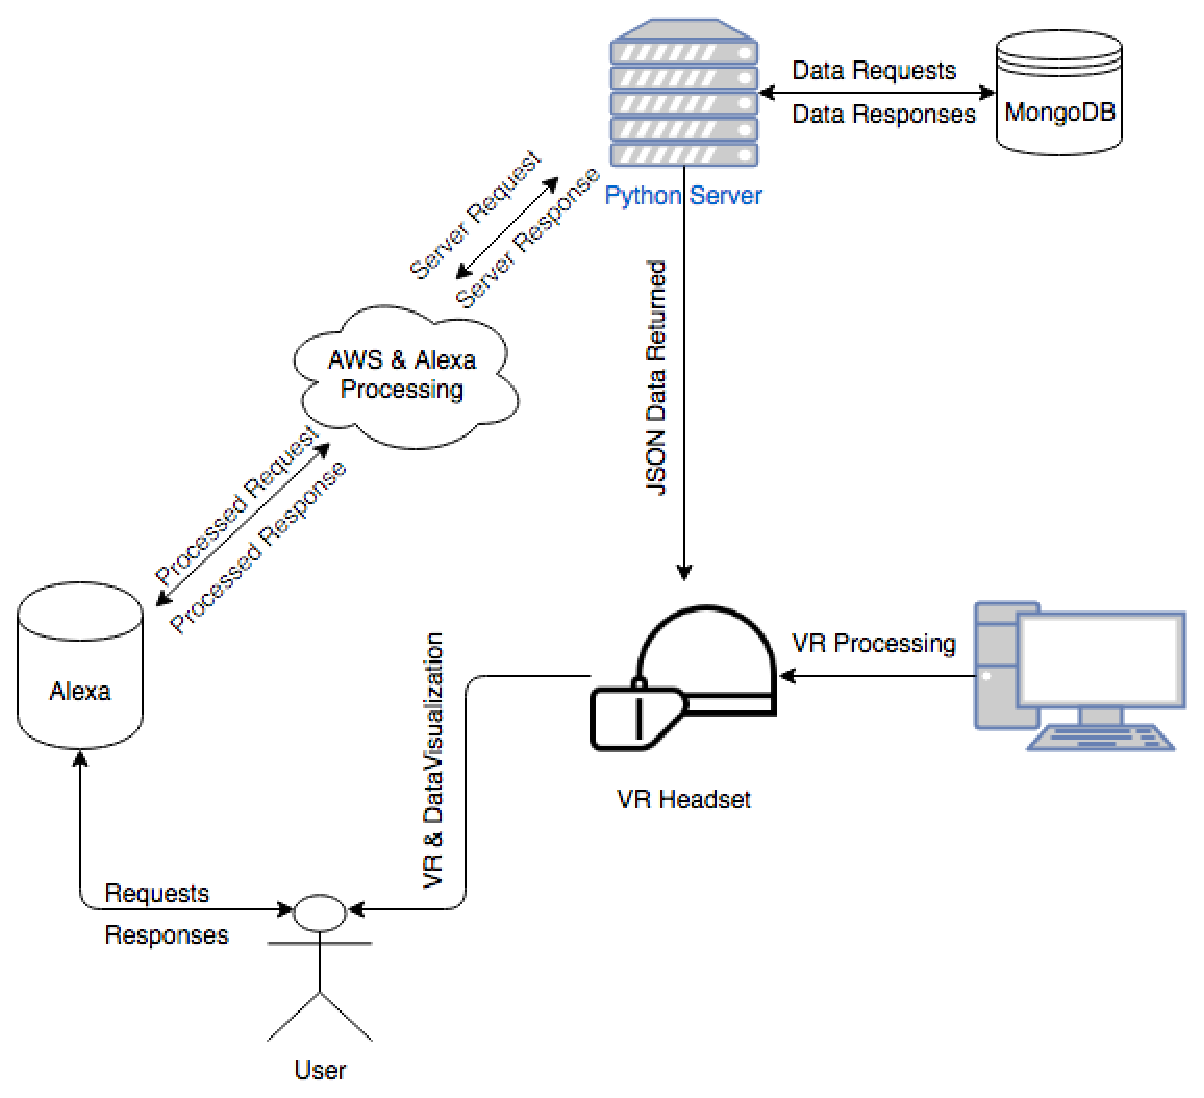
\includegraphics[width=0.5\textwidth]{Design_flow_chart.eps}
            \caption{Overview of complete system architecture}
            \label{fig:design flow chart}
        \end{figure}

    \subsection{Decomposition}
        Through each medium that is passed through, there is a natural decomposition between parts. For example, the Alexa{'}s sole job is to interpret the speech and give the user feedback on whether the action was completed successfully or not. The AWS processes the speech request and sends a request to the proper route on the database. The Python server is used as a method to query data from the database.
        
        To request different amounts of data, the user will specify keywords when talking to Alexa such as maker, type, or date. AWS Lambda will break down the speech response from the Alexa and build the string of words into a route to access on the server. This then makes the proper MongoDB query to get the relevant data from the database and send it to the VR headset to populate the new environment.
        
        \begin{figure}
            \centering
            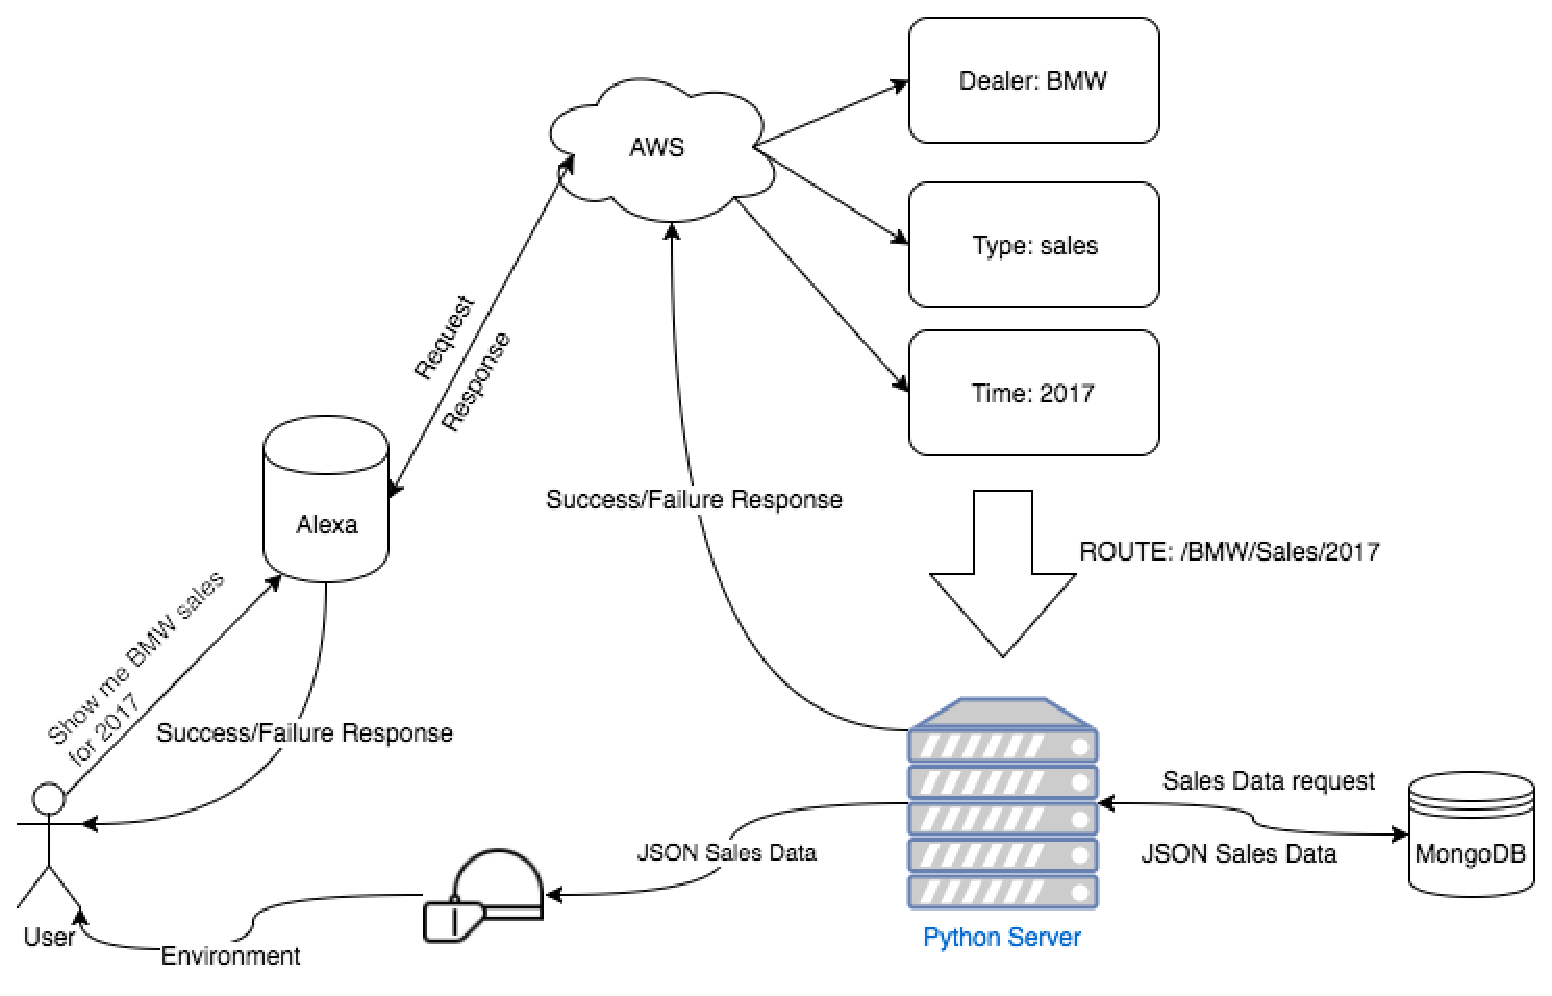
\includegraphics[width=0.5\textwidth]{Alexa_requests.eps}
            \caption{Overview of data flow}
            \label{fig:alexa requests}
        \end{figure}
        
    \subsection{Rationale}
        The overall goal of this project is to try and introduce a new way of computing. Thus, introducing a completely new set of interactions to get data from a computer while feeling natural. The user should only really interact with either their voice and the Alexa, or hand gestures within VR. 
        
        Maintaining a modular design within the system reduces component complexity and eases future development. By reducing the number of roles a component handles, the implementation requirements of that component become considerably lower, which in turn results in clearer, simpler, and more efficient components. A modular system makes implementation of future functionality much more straightforward. Rather than requiring a large redesign of core components, a new module can be included with only minor modifications to an existing codebase.


\section{Perspective}
    \subsection{Stakeholders \& Concerns}
        Per our client{'}s request, the entire project should encompass a modular and object-oriented developmental design, where adding features is an easy thing to implement. This is necessary due to the need for future development within CDK once this capstone project is completed.
        
        Concerning the user, trying to learn a new type of computing method should still feel natural. Thus, normal English language should be used to make requests to the Alexa. Such as, “show me BMW sales data in the US for 2017”, to be followed up by, “now show me the data in Oregon”. Refining the data selection further from the initial request for BMW sales data. At no point should the user actually feel like they are talking to a robot and giving out rudimentary commands.
        
        \begin{figure}
            \centering
            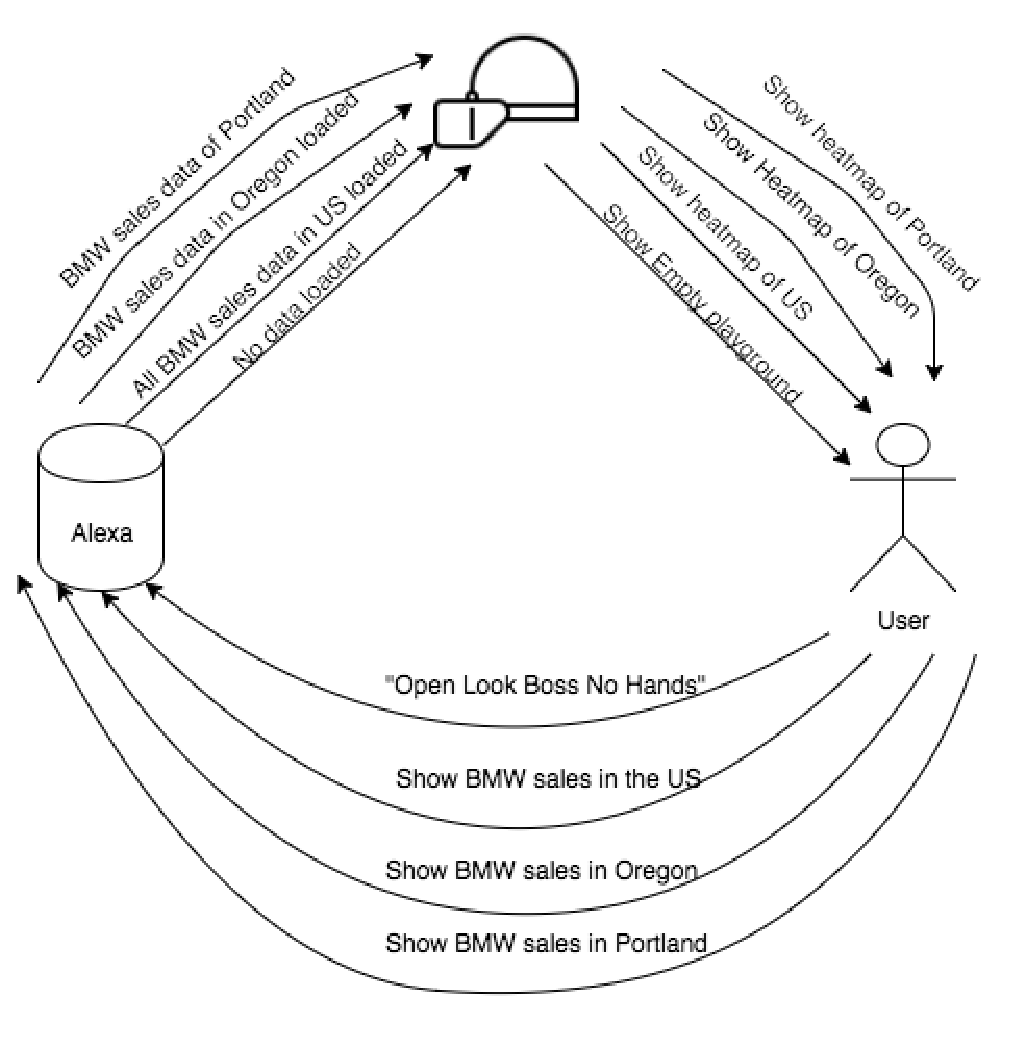
\includegraphics[width=0.5\textwidth]{VR_diagram.eps}
            \caption{A basic modeling of the user menu}
            \label{vr diagram}
        \end{figure}
        
        When making commands, a user should get proper feedback, both from a new environment in VR and audible feedback from the Alexa that their request was successfully or unsuccessfully completed. 
        
        Refinable search queries example of moving from all the US, to just Oregon, to just Portland.
        
        \begin{figure}
            \centering
            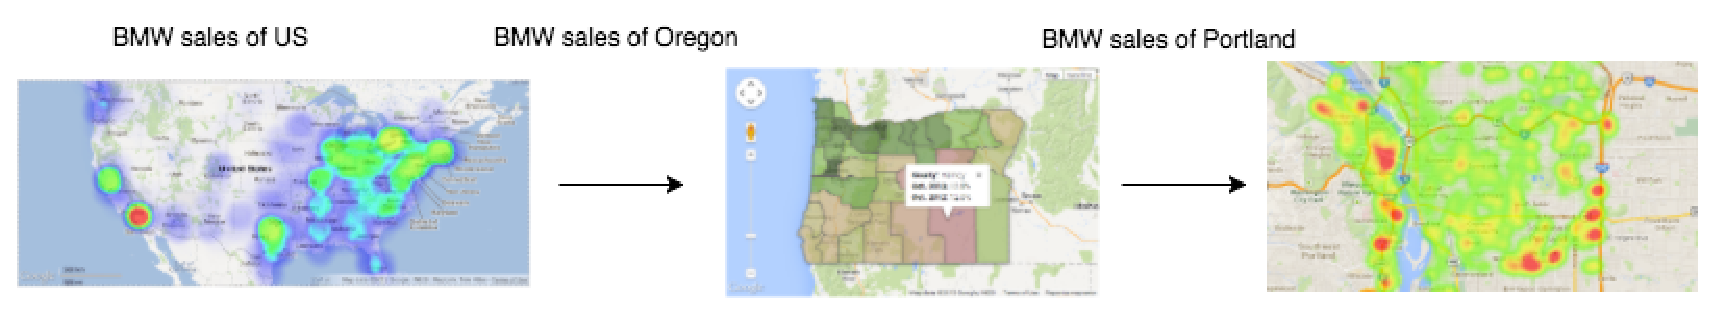
\includegraphics[width=1\textwidth]{Map_diagram.eps}
            \caption{Map refining example}
            \label{fig:map}
        \end{figure}


    \subsection{Design Viewpoints}
        \subsubsection{Context}
            When designing the components for this project, it is important to ensure that they create a suitable abstraction for the user experience. Users with a variety of computer skills may use the system which means the interfaces for both the VR environment and Alexa providing an intuitive experience is crucial.
            
        \subsubsection{Interface}
            Users will require an interface that effectively takes their verbal requests and provides them with a visual representation of the data that is relevant to their request.
            There is also the option of reaching out and grabbing the data, moving it to where the user wants.
            
        \subsubsection{Structure}
            Due to the number of systems that will be utilized, it makes sense to design the components in a modular design. This allows for more efficient and dedicated roles for each module as there is less complexity each one will be responsible for. A modular design has the added benefit of allowing for further module integration later on.
            
        \subsubsection{Interaction}
            The system was designed to require minimal interaction between components to promote modularity and reduce the complexity of each component. 

\section{Components}
    \subsection{Alexa}
        \subsubsection{Interface}
            The Alexa voice assistant requires a request from the user. The requests trigger possible actions, which all send information to the virtual headset for the user to interact with. The user will be able to refine their initial request without needing to reiterate it. 
            
            The only interactions with other hardware Alexa has is the AWS Lambda server, in which it maps what intent and keywords uttered in the phrase to it.

        \subsubsection{Abstractions}
            Amazon{'}s Echo is capable of natural language processing. This means that the echo is actively learning natural conversations and can understand similar phrases, no matter the annunciation or accent. The tutorials Amazon provides for AWS and their developer portal have the ability to change the triggers, the commands and keywords Alexa looks for, and change the intents.

        
        \subsubsection{Structural Elements}
            Session variables will allow for contextual requests by keeping track of what queries were previously requested during the current session and using them to fill in any necessary information that is missing for a given request.
            
            Keyword intents allow for the use of variables within a phrase being uttered to the Alexa. Allowing for a multitude of different meanings that can go into a simple phrase within the same structure.  

        \subsubsection{Design Rationale}
            Amazon{'}s developer portal and AWS website allow the developer to easily create and edit skills. Within the developer portal, you can connect your skill to your designated AWS. The AWS website allows the developer to edit the function code and also the triggers that Alexa will be waiting to hear. Going back to the developer website, they are able to edit details about the skill. They will also be able to add the schema of user intents in JSON format. The developer website is where we connect our developed skill to AWS. The website allows you to test out the skill without a physical Alexa.
        
    \subsection{Communications}
        \subsubsection{Interface}
            No direct interactions to the user. 
            
            The websockets are created by opening up a port inside a computer, in our case it will be on our cloud server. From there, any hardware can connect to the websocket simply by connecting to the port on the computer to receive messages from the server should a new Alexa request need to emit data.

        
        \subsubsection{Abstractions}
            To implement, we will be using websocket packages for Python and C\# to act as a courier for connecting, sending, and receiving messages. The two packages abstract the details of knowing the in{'}s and out{'}s of HTTP protocols. 
            
            To use them, we would be specifying what event/channel name to listen to. From there, when a new message arrives on the channel, an event is fired off in the VR headset say that maps to a custom action. In our case, we will parse the JSON data from the server that was sent within the channel message.
        
        \subsubsection{Structural Elements}
            \begin{itemize}
                \item Channels: What the VR headset subscribes to.
                \item Events: Custom mapping of an action to take after data has been received on the channel. 
                \item Packages: Plug and play websocket functionality between languages.
            \end{itemize}
        
        \subsubsection{Design Rationale}
            There is free and easy to use packages that abstract away all the low level details of HTTP communication from the server to the client. Websockets also offer the benefit of listening for messages on a certain channel, and doing an action when there is new data. Instead of constantly asking the server if anything has changed repetitively.
        
    \subsection{AWS}
        \subsubsection{Interface}
            The interface for users and developers are a multitude of sites from within Amazon that help manage security and accessibility to various parts of cloud computing.
            
            AWS hosts the Python server which sits between Alexa and the data visualization within VR. It works closely with Alexa, allowing the developer to change the function code through the AWS developer website. When requesting data, Alexa sends the request to AWS. Then, AWS queries the database and sends the results to the virtual headset.
        
        \subsubsection{Abstractions}
            AWS provides a way for Amazon{'}s Alexa to interact with the virtual headset through HTTP and cloud computing, including database queries discussed above. AWS also provides a simple text based interface that implements skills created for the Alexa.
        
        \subsubsection{Structural Elements}
            Amazon web services is the cloud computer service and is used by Alexa for intent and language processing. 
            
            AWS also handles the hosting of servers, providing interfaces for accessibility and security.
        
        \subsubsection{Design Rationale}
            AWS is an important component of our project, because it provides the server where the database is queried after requested from Alexa and before sending the results to the HTC Vive. Along with providing language processing and Alexa intent development.
        
    \subsection{Python Server}
        \subsubsection{Interface}
            The Python server interacts with a number of other components. Requests are provided by the Alexa and AWS Lambda which it takes and requests relevant queries  from the database. The returned data is sent to the HTC Vive via the websocket to later be used with data visualization for the user to experience. 
        
        \subsubsection{Abstractions}
            The python server provides an abstraction layer for converting a request from AWS Lambda into a database query, to be sent to the HTC Vive.
        
        \subsubsection{Structural Elements}
            The python server is hosted on AWS to provide a robust and centralized platform for the Alexa, Python, and database interactions. It uses HTTP requests to receive requests from the AWS Lambda, PyMongo to communicate with the database, and websockets to send the data to the VR headset.
        
        \subsubsection{Design Rationale}
            The Python server reduces the amount of work that must be done by AWS Lambda  and the HTC Vive. It provides the developer with a simple interface for turning a request from the Alexa into a JSON object that can be sent down to the headset for the user.
        
    \subsection{Database }
        \subsubsection{Interface}
            The database is interfaced with by the Python server to retrieve the verbal data requested by the user. This is done through the querying and aggregation functionality provided by the MongoDB framework.
            
            The user does not see or interact with the database directly, but instead sees the results of it through the returned data.
        
        \subsubsection{Abstractions}
            The database provides an abstraction layer that facilitates the storage and retrieval of data. This is done through the provided database query framework.
        
        \subsubsection{Structural Elements}
            The database is built upon MongoDB. This provides a JSON like data format that is well suited for working with queries provided through an Amazon Alexa intent.
        
        \subsubsection{Design Rationale}
            The database creates an efficient and straightforward method for the developers to store and access data. 
            
            Along with MongoDB{'}s aggregation pipeline, it allows for easy queries that nearly mirror natural language when trying to filter through documents. 
        
    \subsection{Virtual Reality}
        \subsubsection{Interface}
            The headset should be able to view the data visualization through virtual reality. Through the use of hand-held controllers, the user will be able to interact with the displayed data to change the display aspects, such as size and location.
        
        \subsubsection{Abstractions}
            The virtual reality component will create an abstraction layer for the visual display and interaction of data.
        
        \subsubsection{Structural Elements}
            The virtual reality environment is created using the Unity3D engine and a HTC Vive. 
            
            Inside the Unity3D engine, programmatically one can create GameObjects to items which can then have attributes added to them such as color, texture, or interaction method.
        
        \subsubsection{Design Rationale}
            Virtual reality is one of the key components of the project, it is the final destination for the user{'}s requested data. From a user{'}s perspective, they will see the information they asked for.
        
    \subsection{Data Visualization}
        \subsubsection{Interface}
            The user should be able to view the data in classic ways such as bar charts, pie charts, and heatmaps. 
            
            They interface with the software by being a GameObject in the Unity environment.
        
        \subsubsection{Abstractions}
            These graphs and charts will have an abstraction layer around them, such that the only thing that they care about are numbers corresponding to a certain field to be displayed. 
            Via the Unity engine, these graphs and maps will be presented to a user in 3D as objects the can reach out and touch.

        
        \subsubsection{Structural Elements}
            Each type of data visualization will be contained inside it{'}s own file, and object. 
            GameObject attributes for adding VR methods and interactivity to the graphs.
        
        \subsubsection{Design Rationale}
            Data visualization provides users with a variety of ways to view the data. These views can highlight trends that might otherwise be missed from looking at just raw data.
        
    \subsection{VR Interactions}
        \subsubsection{Interface}
            VR interactions take movements from the hand-held controls and communicate them to the VR system to change the display properties.
        
        \subsubsection{Abstractions}
            VR interaction abstract away the details of the display properties within the VR environment and allows the user to modify the display physically.
        
        \subsubsection{Structural Elements}
            Using the Unity engine, the displayed GameObjects contain attributes that can be modified in near real-time to change their appearance in VR.
        
        \subsubsection{Design Rationale}
            In VR the user has limited access to standard controls such as a keyboard or mouse. This requires an alternate method for providing display adjustments. This is provided through the use of the precise hand-held controls.

\section{VR User Interface}
    \subsection{Overview}
        The user should be placed inside a virtual room with a cylindrical table in the middle, when the user interacts with the table, a flat plane comes out from the table giving the user the heatmap of nonspecific sales data. The user will then have the ability to either ask Alexa to refine the data down by state, or time. If the user so chooses, they can also reach out and touch the map as to where they want to refine the data. 
        To the left and right of the virtual plane will be different data visualizations of the current state of the map.
        \begin{figure}
            \centering
            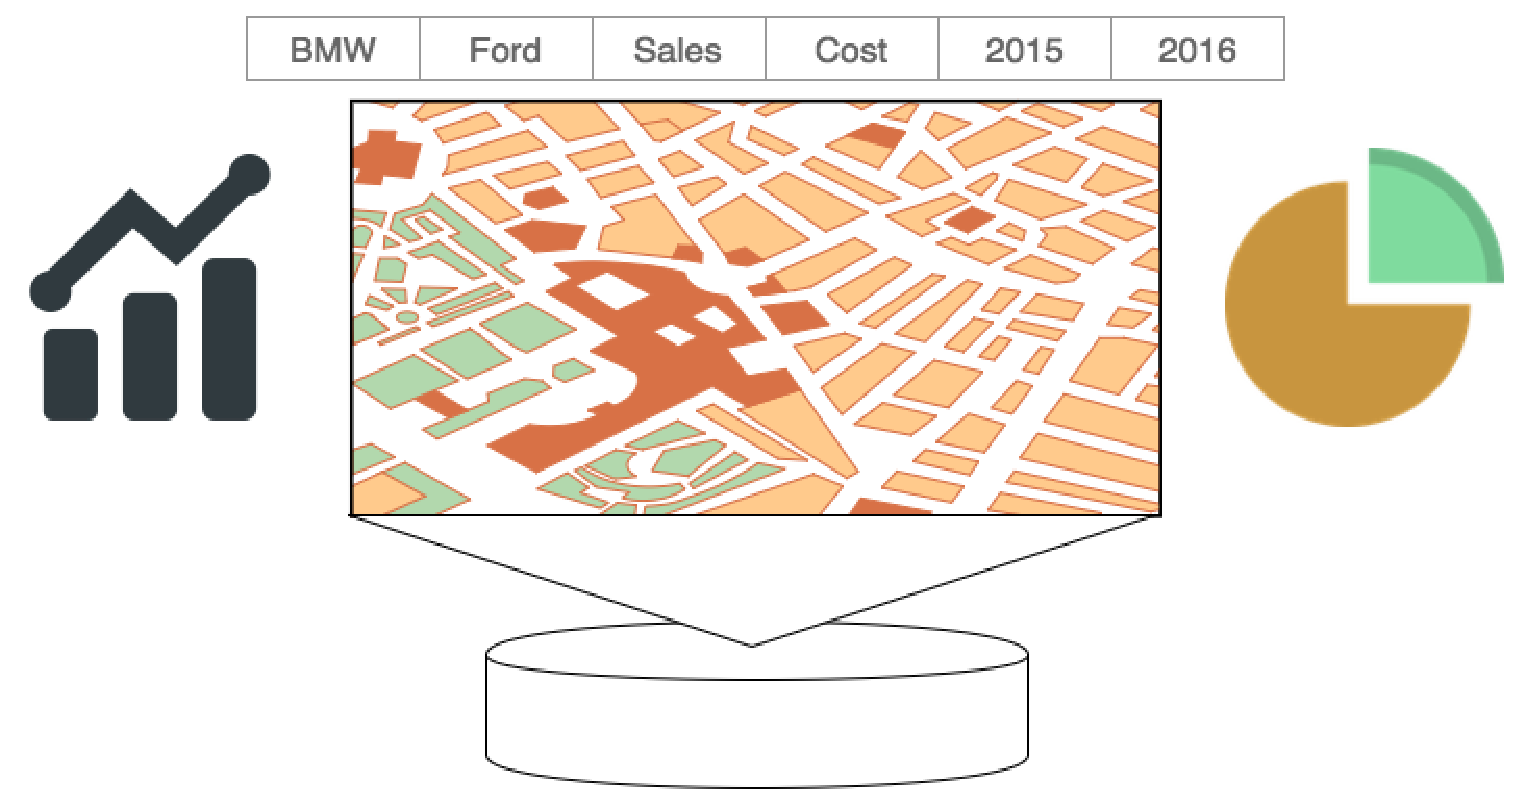
\includegraphics[width=0.5\textwidth]{Basic_interaction.eps}
            \caption{Visual overview of the basic layout for mapping and graphing}
            \label{fig:Data visualization layout}
        \end{figure}
    
    \subsection{Navigation}
        A user should be able to move around the virtual room by moving their controllers in a running-like motion. Or by pointing at a section of the room and pressing a designated button to teleport to where they would like to go.
    
    \subsection{Interaction}
        Requesting and accessing additional or reduced data will be performed through commands told to the Alexa. Or, by pointing at an object/figure with a laser pointer from their controller.

\section{Development Stages}
    \begin{enumerate}
        \item Acquire all the proper hardware and software (HTC Vive, Amazon Alexa, game engine, etc). 
        \item Set up all project related software (Github, IM channel, server hosting, etc).
        \item Create sprint stories, epics, and estimations.
        \item Stand up an instance of MongoDB, and the Python cloud server. 
        \item Create basic Alexa intents and request/response processing.
        \item Such that Alexa repeats back what you have said, or some other hard coded phrase, upon a certain request. 
        \item Generate fake data for MongoDB.
        \item With a computer script to maintain data integrity. 
        \item Add functionality for Alexa to connect to the cloud server and go to a Python server route to get a unique response back. 
        \item Build a blank playground in virtual reality
        \item Connect Alexa to retrieve database records from server.
        \item Implement data return from server to VR by Alexa command
        \item Create interactive map in VR 
        \item Refine from country, to state, to city.
        \item Implement data visualization in VR
        \item Retrieving data from the server, display it in the form of bar or pie charts. 
        \item Connect the current map state to the Alexa, and have it change appropriately in VR .
        \item Connect the current map state to the proper data visualization 
        \item Implement ability to refine or change data visualization within VR.
    \end{enumerate}

\end{document}